\documentclass{article}\usepackage[]{graphicx}\usepackage[]{color}
% maxwidth is the original width if it is less than linewidth
% otherwise use linewidth (to make sure the graphics do not exceed the margin)
\makeatletter
\def\maxwidth{ %
  \ifdim\Gin@nat@width>\linewidth
    \linewidth
  \else
    \Gin@nat@width
  \fi
}
\makeatother

\definecolor{fgcolor}{rgb}{0.345, 0.345, 0.345}
\newcommand{\hlnum}[1]{\textcolor[rgb]{0.686,0.059,0.569}{#1}}%
\newcommand{\hlstr}[1]{\textcolor[rgb]{0.192,0.494,0.8}{#1}}%
\newcommand{\hlcom}[1]{\textcolor[rgb]{0.678,0.584,0.686}{\textit{#1}}}%
\newcommand{\hlopt}[1]{\textcolor[rgb]{0,0,0}{#1}}%
\newcommand{\hlstd}[1]{\textcolor[rgb]{0.345,0.345,0.345}{#1}}%
\newcommand{\hlkwa}[1]{\textcolor[rgb]{0.161,0.373,0.58}{\textbf{#1}}}%
\newcommand{\hlkwb}[1]{\textcolor[rgb]{0.69,0.353,0.396}{#1}}%
\newcommand{\hlkwc}[1]{\textcolor[rgb]{0.333,0.667,0.333}{#1}}%
\newcommand{\hlkwd}[1]{\textcolor[rgb]{0.737,0.353,0.396}{\textbf{#1}}}%
\let\hlipl\hlkwb

\usepackage{framed}
\makeatletter
\newenvironment{kframe}{%
 \def\at@end@of@kframe{}%
 \ifinner\ifhmode%
  \def\at@end@of@kframe{\end{minipage}}%
  \begin{minipage}{\columnwidth}%
 \fi\fi%
 \def\FrameCommand##1{\hskip\@totalleftmargin \hskip-\fboxsep
 \colorbox{shadecolor}{##1}\hskip-\fboxsep
     % There is no \\@totalrightmargin, so:
     \hskip-\linewidth \hskip-\@totalleftmargin \hskip\columnwidth}%
 \MakeFramed {\advance\hsize-\width
   \@totalleftmargin\z@ \linewidth\hsize
   \@setminipage}}%
 {\par\unskip\endMakeFramed%
 \at@end@of@kframe}
\makeatother

\definecolor{shadecolor}{rgb}{.97, .97, .97}
\definecolor{messagecolor}{rgb}{0, 0, 0}
\definecolor{warningcolor}{rgb}{1, 0, 1}
\definecolor{errorcolor}{rgb}{1, 0, 0}
\newenvironment{knitrout}{}{} % an empty environment to be redefined in TeX

\usepackage{alltt}

\usepackage{float}

% Set the margins on the page to not be so large
\addtolength{\oddsidemargin}{-.875in}
\addtolength{\evensidemargin}{-.875in}
\addtolength{\textwidth}{1.75in}
\addtolength{\topmargin}{-.875in}
\addtolength{\textheight}{1.75in}

% Take off page numbering
\pagenumbering{gobble}
\IfFileExists{upquote.sty}{\usepackage{upquote}}{}
\begin{document}

\title{%
  2.4.1: SAS - Simultaneous Inference and Regression Through Origin \\
  \smallskip
  \large Stat 5100: Dr. Bean
}
\date{}

\maketitle

\textbf{Example: } Toluca dataset

\begin{knitrout}
\definecolor{shadecolor}{rgb}{0.969, 0.969, 0.969}\color{fgcolor}\begin{kframe}
\begin{alltt}
\hlcom{# Input data}
\hlkwd{library}\hlstd{(stat5100)}
\hlkwd{data}\hlstd{(toluca)}

\hlcom{# Create linear model and obtain 95% confidence interval of beta parameters,}
\hlcom{# but this time use the simultaneous comparison adjustment}
\hlstd{toluca_lm} \hlkwb{<-} \hlkwd{lm}\hlstd{(workhours} \hlopt{~} \hlstd{lotsize,} \hlkwc{data} \hlstd{= toluca)}
\hlstd{stat5100}\hlopt{::}\hlkwd{coefficient_confidence_lm}\hlstd{(toluca_lm,} \hlkwc{confidence} \hlstd{=} \hlnum{0.95}\hlstd{,} \hlkwc{simul} \hlstd{=} \hlnum{TRUE}\hlstd{)}
\end{alltt}
\begin{verbatim}
## lower.est and upper.est are the 97.5% confidence limits.
## The Bonferroni adjustment for simultaneous confidence levels was made.
##              Estimate Std. Error   t value     Pr(>|t|)  lower.est  upper.est
## (Intercept) 62.365859 26.1774339  2.382428 2.585094e-02 -0.4043574 125.136075
## lotsize      3.570202  0.3469722 10.289592 4.448828e-10  2.7382061   4.402198
\end{verbatim}
\end{kframe}
\end{knitrout}

\subsection*{Simultaneous 90\% interval estimation of mean workhours (Bonferroni and Working-Hotelling)}
\begin{knitrout}
\definecolor{shadecolor}{rgb}{0.969, 0.969, 0.969}\color{fgcolor}\begin{kframe}
\begin{alltt}
\hlstd{toluca_sites_A} \hlkwb{<-} \hlkwd{data.frame}\hlstd{(}\hlkwc{lotsize} \hlstd{=} \hlkwd{c}\hlstd{(}\hlnum{30}\hlstd{,} \hlnum{65}\hlstd{,} \hlnum{100}\hlstd{))}
\hlstd{stat5100}\hlopt{::}\hlkwd{simul_mean_prediction_limits}\hlstd{(toluca_lm, toluca_sites_A,} \hlkwc{confidence} \hlstd{=} \hlnum{0.90}\hlstd{)}
\end{alltt}
\begin{verbatim}
##   lotsize     yhat   se_yhat WH_lower WH_upper  B_lower  B_upper
## 1      30 169.4719 16.969741 131.1542 207.7897 131.0570 207.8868
## 2      65 294.4290  9.917579 272.0351 316.8229 271.9783 316.8797
## 3     100 419.3861 14.272328 387.1591 451.6130 387.0774 451.6947
\end{verbatim}
\end{kframe}
\end{knitrout}


\subsection*{Simultaneous 95\% prediction limits for two lots (Bonferroni and Scheffe)}
\begin{knitrout}
\definecolor{shadecolor}{rgb}{0.969, 0.969, 0.969}\color{fgcolor}\begin{kframe}
\begin{alltt}
\hlstd{toluca_sites_B} \hlkwb{<-} \hlkwd{data.frame}\hlstd{(}\hlkwc{lotsize} \hlstd{=} \hlkwd{c}\hlstd{(}\hlnum{80}\hlstd{,} \hlnum{100}\hlstd{))}
\hlstd{stat5100}\hlopt{::}\hlkwd{simul_prediction_limits}\hlstd{(toluca_lm, toluca_sites_B,} \hlkwc{confidence} \hlstd{=} \hlnum{0.95}\hlstd{)}
\end{alltt}
\begin{verbatim}
##   lotsize     yhat se_yhat_pred  S_lower  S_upper  B_lower  B_upper
## 1      80 347.9820     49.91095 217.4073 478.5568 228.3018 467.6622
## 2     100 419.3861     50.86664 286.3111 552.4610 297.4142 541.3579
\end{verbatim}
\end{kframe}
\end{knitrout}

\subsection*{Regression through origin example}

This dataset is called ``warehouse'': a plumbing supplies company that is looking at the relation between work units (X) and labor costs (Y) at its 12 warehouses.

\begin{knitrout}
\definecolor{shadecolor}{rgb}{0.969, 0.969, 0.969}\color{fgcolor}\begin{kframe}
\begin{alltt}
\hlkwd{data}\hlstd{(warehouse)}
\hlkwd{head}\hlstd{(warehouse)}
\end{alltt}
\begin{verbatim}
##   work cost
## 1   20  114
## 2  196  921
## 3  115  560
## 4   50  245
## 5  122  575
## 6  100  475
\end{verbatim}
\begin{alltt}
\hlcom{# Fit a linear model through the origin}
\hlstd{warehouse_lm_origin} \hlkwb{<-} \hlkwd{lm}\hlstd{(cost} \hlopt{~} \hlnum{0} \hlopt{+} \hlstd{work,} \hlkwc{data} \hlstd{= warehouse)}

\hlcom{# Look at some statistics}
\hlkwd{anova}\hlstd{(warehouse_lm_origin)}
\end{alltt}
\begin{verbatim}
## Analysis of Variance Table
## 
## Response: cost
##           Df  Sum Sq Mean Sq F value    Pr(>F)    
## work       1 4191980 4191980   18762 < 2.2e-16 ***
## Residuals 11    2458     223                      
## ---
## Signif. codes:  0 '***' 0.001 '**' 0.01 '*' 0.05 '.' 0.1 ' ' 1
\end{verbatim}
\begin{alltt}
\hlkwd{summary}\hlstd{(warehouse_lm_origin)}
\end{alltt}
\begin{verbatim}
## 
## Call:
## lm(formula = cost ~ 0 + work, data = warehouse)
## 
## Residuals:
##     Min      1Q  Median      3Q     Max 
## -24.720  -4.020   4.432  11.141  21.194 
## 
## Coefficients:
##      Estimate Std. Error t value Pr(>|t|)    
## work  4.68527    0.03421     137   <2e-16 ***
## ---
## Signif. codes:  0 '***' 0.001 '**' 0.01 '*' 0.05 '.' 0.1 ' ' 1
## 
## Residual standard error: 14.95 on 11 degrees of freedom
##   (1 observation deleted due to missingness)
## Multiple R-squared:  0.9994,	Adjusted R-squared:  0.9994 
## F-statistic: 1.876e+04 on 1 and 11 DF,  p-value: < 2.2e-16
\end{verbatim}
\begin{alltt}
\hlcom{# What does the fit look like?}
\hlcom{# (R doesn't plot the origin inside of the graph, but only because the data}
\hlcom{# doesn't stretch to the point (0,0). Understand that this plot does have the}
\hlcom{# regression line going through the origin even though it is outside the graph)}
\hlstd{stat5100}\hlopt{::}\hlkwd{fit_plot}\hlstd{(warehouse_lm_origin,} \hlkwc{xlab} \hlstd{=} \hlstr{"work"}\hlstd{,} \hlkwc{ylab} \hlstd{=} \hlstr{"cost"}\hlstd{,}
                   \hlkwc{main} \hlstd{=} \hlstr{"Regression through origin"}\hlstd{)}
\end{alltt}
\end{kframe}

{\centering 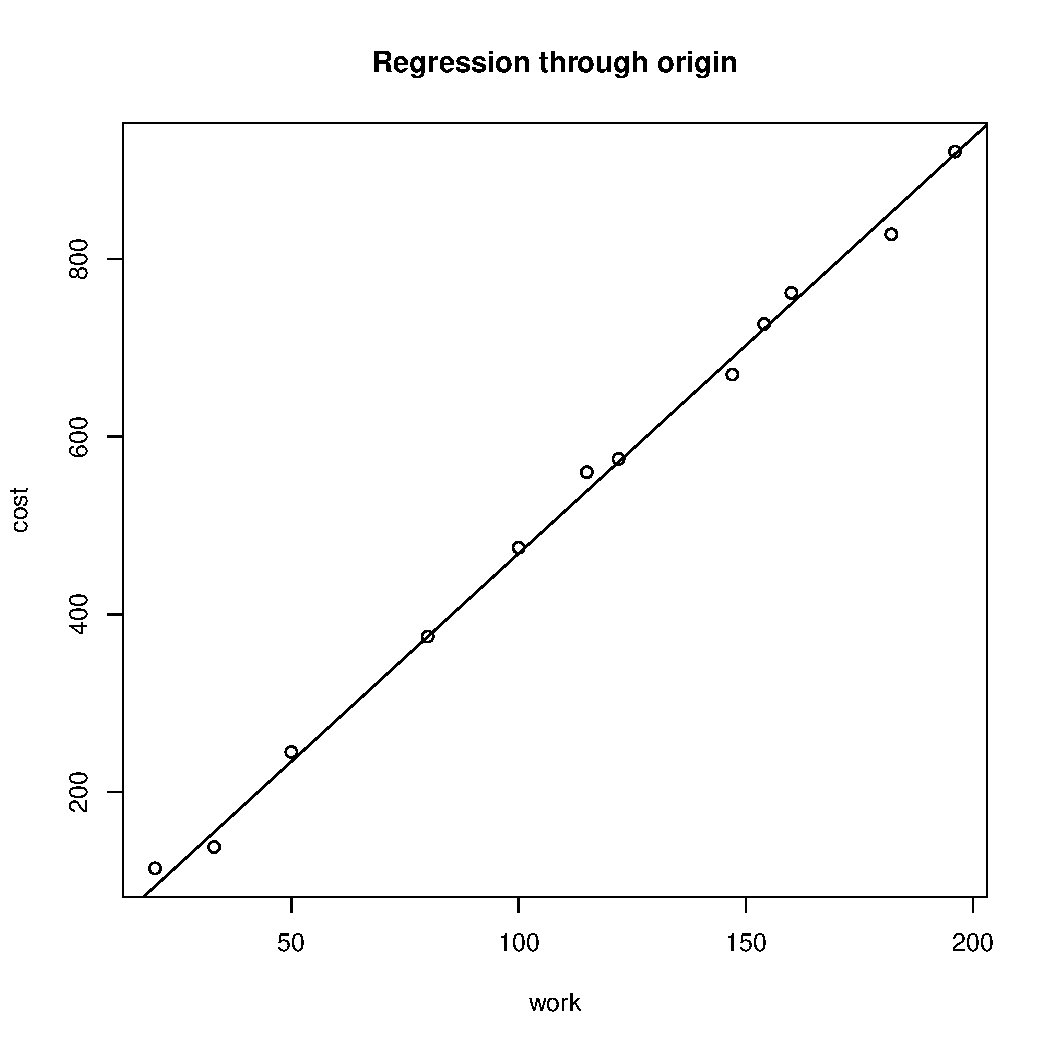
\includegraphics[width=0.6\textwidth]{figure/unnamed-chunk-4-1} 

}



\end{knitrout}


\end{document}
